\chapter{Umsetzung Teilprojekt SAE}

\section{Datenbank}
Dieser Abschnitt fokussiert sich auf die in der Softwarelösung verwendete Datenbank und deren Modellierung. Für die Software wurde eine SQLite Datenbank verwendet.

In der Software wurde das Entity Framework verwendet um Tabellen und Relationen anhand von zuvor definierten Klassen zu generieren. Dazu wurden 4 Klassen angelegt User, Company, Interest und Address, die dann zu Tabellen automatisch umgewandelt werden. Dabei wird aus Attributen wie z.B. der Name von User eine Spalte mit eben dieser Bezeichnung. Außerdem wird der Datentyp passend zum Attribut gewählt. Relationen werden ebenso erzeugt z.B. wenn ein User eine Adresse besitzt und damit ein Attribut vom Typ Address hat.

\subsection{Datenbankmodell}
Betrachten wir zunächst ein ER-Modell der Datenbank um einen Überblick zu erhalten.

\begin{figure}[h]
	\centering
	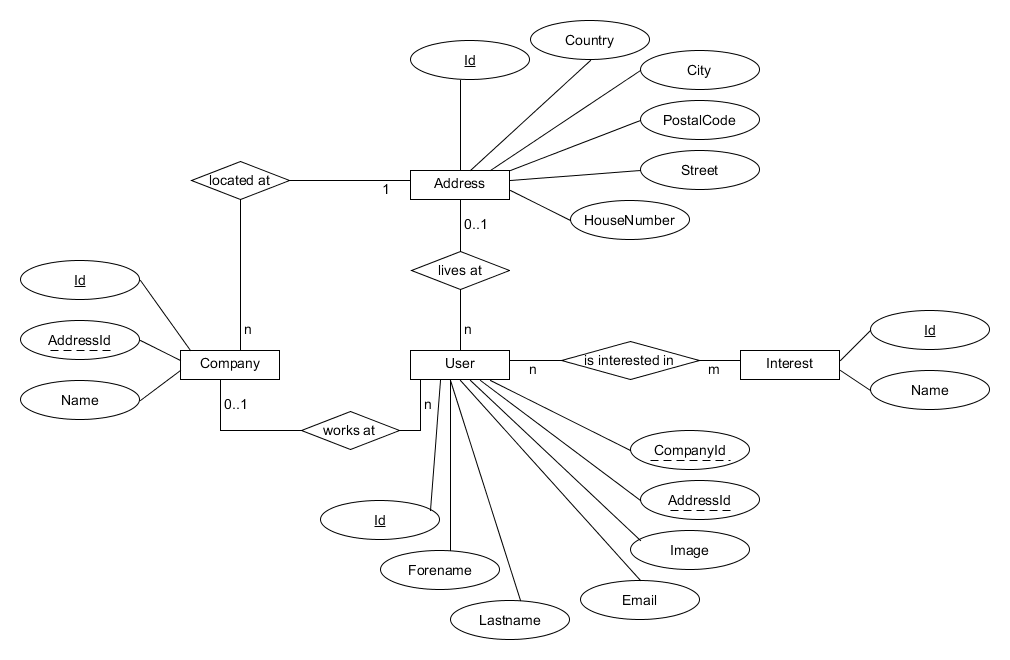
\includegraphics[width=\linewidth]{Images/Projekt_Messe_ERModell2}
	\caption{ER-Modell der Datenbank für die Softwarelösung}
	\label{fig:projektmesseermodell}
\end{figure}

\subsection{Entitäten}
In diesem Abschnitt betrachten wir die Entitäten des ER-Modells und ihre Attribute genauer.

\subsubsection{User}
Die Entität User repräsentiert den Kunden, der seine Daten auf der Messe angegeben hat. Diese Person hat einen Name, Email, Bild, Adresse und eventuell eine Firmenzugehörigkeit. Der Primärschlüssel ist Id, wohingegen AdressId und CompanyId Fremdschlüssel sind.

\subsubsection{Company}
Diese Entität repräsentiert eine Firma, der ein Kunde möglicherweise angehören kann. Sie hat eine Id als Primärschlüssel, einen Namen und eine Adresse mit AddressId als Fremdschlüssel.

\subsubsection{Address}
Die Entität Address hat eine primäre Id, Land, Stadt, Postleitzahl, Straße und Hausnummer.

\subsubsection{Interest}
Eine Interesse hat eine primäre Id und einen Namen.

\subsection{Relationen}

\subsubsection{Company - Address}
Eine Firma hat genau eine Adresse wohingegen an einem Standort auch mehrere Firmen angesiedelt sein können. Dies wird die gezeigte 1:n Relation widergespiegelt. Der Verweise von der Firma auf die Adresse wird mit Hilfe des Fremdschlüssels AddressId gelöst.

\subsubsection{User - Address}
Ein Kunde hat eine oder keine Adresse, wohingegen an einem Ort durchaus mehrere Leute wohnen können. Diese 1:n Relation wird durch den Fremdschlüssel AddressId modelliert.

\subsubsection{User - Company}
Ein Kunde kann Mitarbeiter einer Firma sein, muss es aber nicht und eine Firma kann viele Mitarbeiter haben. Diese 1:n Relation wird durch den Fremdschlüssel CompanyId modelliert.

\subsubsection{User - Interest}
Ein Kunde kann mehrere Interessen haben, aber eine Interesse wie z.B. Reisen kann von vielen Kunden favorisiert werden. Diese n:m Relation wird durch zwei Listen gelöst, wovon sich jeweils eine in der Entität User und Interest befindet.

\section{Aufbau und Funktionsweise}
\subsection{Architektur}
\subsection{USE Case und UML Diagramme}
\subsection{Prerequisites: Bibliotheken und Komponenten}
\subsection{Inbetriebnahme vor Ort}
\subsection{Technische Beschreibung der WebCam Anbindung}
\subsection{Anleitung Bedienung durch den Kunden}
\subsection{Anleitung Datenabruf und Übermittlung}
\subsection{Testszenarien}

